\chapter{[SKE] Spolehlivost komponentních systémů, redundantní struktury, důležitost komponent.}

% lecture 7
    \begin{define}
        Předpokládejme, že máme systém o $n$ komponentách. Budeme charakterizovat stav $i$-té komponenty $x_i$ binárně jako funguje/nefunguje, tedy $x_i\in\{0,1\}$. Označme $\textbf{x}=(x_1,...,x_n)$ jako \textbf{stavový vektor}. 
        
        Předpokládejme, že známe-li $\textbf{x}$, pak známe stav celého systému $S$, tzn. jsme schopni definovat \textbf{strukturní funkci} $\crossedphi(\textbf{x})=\begin{cases}
        1,&\text{systém funguje,}\\0,&\text{systém nefunguje.}
        \end{cases}$
    \end{define}

    Tímto způsobem můžeme zkoumat různě zapojené součásti, třeba sériově, 
    paralelně (jsou tedy v redundanci) apod. U sériového zapojení stačí 
    jedna vadná součástka, aby systém přestal fungovat a u paralelního 
    systému stačí, když alespoň jedna součástka funguje, aby systém 
    fungoval. Pozor ale, že záleží na reprezentaci, někdy se např. sériově 
    zapojené součástky chovají, jako by byly paralelní (např. ventily na 
    potrubí, aby voda netekla, alespoň jeden ventil musí fungovat).

    \begin{corollary}
        Logické zapojení komponent se může zakreslit pomocí blokových diagramů (RBD - Reliability Block Diagram) (podobné elektrickému zapojení). Pro sériově zapojené součásti máme 
        $$ \crossedphi(\textbf{x})=\prod_{i=1}^{n}x_i=\min(x_i)_1^n.$$
        Paralelně zapojené součástky pak
        $$ \crossedphi(\textbf{x})=1-\prod_{i=1}^{n}(1-x_i)\equal{ozn}\bigsqcup_{i=1}^n x_i=\max(x_i)_1^n, $$ kde $\bigsqcup$ označuje inverzní produkt.
    \end{corollary}

    \begin{define}[k-o-o-n struktura]
        k-o-o-n struktura (k-out-of-n) je taková, že systém funguje, pokud je alespoň $k$ z komponent je funkční. Potom
        $$ \crossedphi(\textbf{x})=\begin{cases}
        1,&\text{pokud }\sumin x_i\geq k,\\0,& \text{jinak.}
        \end{cases}$$
        Tento systém se může použít třeba pro přivolávání hasičů, pokud 2oon zaznamenají kouř. Tímto se eliminují false positive chyby ve stylu zapálená cigareta apod. Například systém 2oo3 se dá zapsat jako paralelní vlákna $\{(1,2), (2,3),(1,3)\}$. Není to však jediná možnost, viz obrázek \ref{fig:2oo3}.
        
        \begin{figure}[h]
            \centering
            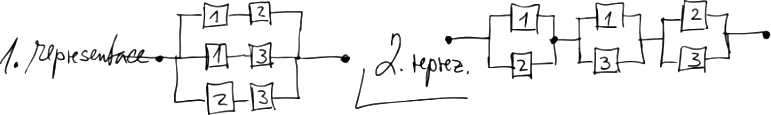
\includegraphics[width=0.7\linewidth]{pictures/2oo3}
            \caption{Dvě možnosti zapojení systému 2oo3, paralelní systém minimálnních cest (vlevo) a série minimálních řezů (vpravo).}
            \label{fig:2oo3}
        \end{figure}
        
        Máme tedy $\crossedphi(\textbf{x})=x_1x_2\bigsqcup x_1x_3\bigsqcup x_2x_3$
    \end{define}

    \begin{theorem}
        Mějme systém S o $n$ komponentech. Mějme dále minimální cesty $P_1,...,P_k$ (funkční cesty ze kterých nelze nic odstranit). Pak $$ \crossedphi(\textbf{x})=\bigsqcup_{j=1}^k \prod_{i\in P_j} x_i.$$
        Naopak z minimálních řezů $K_1,...,K_l$ můžeme dostat
        $$ \crossedphi(\textbf{x})= \prod_{j=1}^k \bigsqcup_{i\in K_k} x_i.$$
        V praxi pak používáme ten vzorec, který nejvíce zjednodušuje výpočet.
    \end{theorem}

    \begin{corollary}
        Definujeme strukturu BRIDGE (viz obr. \ref{fig:bridge}). Tady máme 4 cesty, kudy projít, tedy $\{(1,2),(4,5),(1,3,5),(4,3,2)\}$. Z toho můžeme udělat $\crossedphi(\textbf{x})$. Poměrně jednoduše se dá udělat i diagram řezů.
        
        \begin{figure}[h]
            \centering
            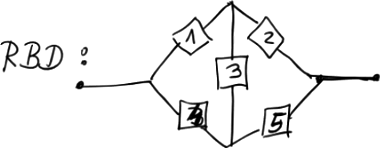
\includegraphics[width=0.3\linewidth]{pictures/bridge}
            \caption{Strukture BRIDGE.}
            \label{fig:bridge}
        \end{figure}
        
    \end{corollary}

    \begin{theorem}[Pivotální rozklad]
        Mějme systém $S$ o $n$ komponentách. Pak můžeme $\crossedphi(\textbf{x})$ rozepsat jako 
        $$\crossedphi(\textbf{x})=x_i\crossedphi(1_i,\textbf{x}_{-i})+(1-x_i)\crossedphi(0_i,\textbf{x}_{-i}),$$
        kde fixujeme, že $i$-tý prvek funguje/nefunguje. Tento rozklad se může použít rekurentně až do 
        $$\crossedphi(\textbf{x})=\sum_{\textbf{y}}\prod_{j=1}^n x_j^{y_j}(1-x_j)^{1-y_j}\crossedphi(\textbf{y}),$$ kde $\textbf{y}$ jsou $n$-rozměrné binární vektory, kterých je $2^n$.
    \end{theorem}

    Toto se hodí např. pro BRIDGE, kde je ideální udělat rozklad podle prvku 3. Potom dostaneme 
    $$ \crossedphi(\textbf{x})=x_3\crossedphi(1_3,\textbf{x}_{-3})+(1-x_3)\crossedphi(0_3,\textbf{x}_{-3}). $$ 
    Tím se výrazně zjednoduší struktura systému.

    \begin{define}[Strukturní důležitost komponent]
        Stavový vektor $(1_i,\textbf{x})$ se nazývá \textbf{kritická cesta/vektor pro $i$-tou komponentu}, pokud $\crossedphi(1_i,\textbf{x})=1\wedge \crossedphi(0_i,\textbf{x})=0 $, tzn. $\crossedphi(1_i,\textbf{x})-\crossedphi(0_i,\textbf{x})=1$.
        
        Označme $\eta_\crossedphi(i)=\sum_{(\cdot_i,\textbf{x}_{-i})} \big[\crossedphi(1_i,\textbf{x})-\crossedphi(0_i,\textbf{x})\big]$ počet kritických vektorů pro $i$-tou komponentu.
        
        Číslo $B_\crossedphi(i)=\frac{\eta_\crossedphi(i)}{2^{n-1}}$ nazveme \textbf{Birmbaumova míra (strukturní) důležitosti} $i$-té komponenty v $S$.
    \end{define}

    \begin{example}
        Komponenta 1 je v sérii s paralelní 2 a 3. Pak pro $i=1$ dostaneme
        $$\begin{array}{c|c}
            (\cdot,x_2,x_3) & \crossedphi(1_i,\textbf{x})-\crossedphi(0_i,\textbf{x})=1 \\\hline
            \cdot\,00 & 0 \\
            \cdot\,01 & 1 \\
            \cdot\,10 & 1 \\
            \cdot\,11 & 1 
        \end{array}.$$
        Jelikož $2^{n-1}=4$, pak $\eta_\crossedphi(1)=3$, takže $B_\crossedphi(1)=\frac{3}{4}$ apod.
        
    \end{example}


    \begin{define}
        $i$-tá komponenta se nazývá \textbf{irelevantní}, pokud $\crossedphi(1_i,\textbf{x})=\crossedphi(0_i,\textbf{x})$, $\forall\textbf{x}_{-i}$. Tedy že na jejím vypnutí/zapnutí nezáleží. Příkladem je záznamové zařízení při požárním poplachu, které je sice důležité, ale na samotný poplach nemá vliv.
    \end{define}

    \begin{define}
        Systém komponent se nazývá \textbf{koherentní}, pokud neobsahuje irelevantní komponenty a strukturní funkce je neklesající v každé své proměnné.
    \end{define}

    \begin{theorem}
        Pro $S$ koherentní platí, že $\crossedphi(\textbf{0})=0$, $\crossedphi(\textbf{1})=1$ a $$ \prod_{i=1}^n x_i\leq \crossedphi(\textbf{x})\leq \bigsqcup_{i=1}^n x_i. $$
    \end{theorem}

    \begin{define}[Spolehlivostní funkce]
        Pro výpočet $R_S(t)$ využijeme čas $t$ a ztotožníme poruchovostní komponenty 
        $$X_i(t)=\begin{cases}1,&\text{s pravděpodobností }p_i=\PP(T_i>t),\\0,&\text{jinak.}\end{cases}$$
        Dosazením do strukturní funkce potom vyrobíme $\crossedphi\big(\textbf{X}(t)\big)$, kde $\textbf{X}(t)$ je vektor veličin $X_i(t)$, které charakterizují funkčnost/nefunkčnost komponenty v čase $t$. Potom
        $$ R_S(t)=\PP(T_S>t)=\PP\big(\crossedphi\big(\textbf{X}(t)\big)=1\big)=1\cdot\PP\big(\crossedphi\big(\textbf{X}(t)\big)=1\big)+0\cdot\PP\big(\crossedphi\big(\textbf{X}(t)\big)=0\big)=\EE{\crossedphi\big(\textbf{X}(t)\big)}. $$
    \end{define}

    \begin{example}
        Pro sériově zapojený $S$ dostaneme
        $$ R_S(t)=\E \crossedphi\big(\textbf{X}(t)\big)\equal{id}\prod_{i=1}^n \E X_i(t)=\prod_{i=1}^n R_i(t)=\prod_{i=1}^n \e{-\int_{0}^{t}\lambda_i(\tilde{t})\d\tilde{t}}=\e{-\int\limits_{0}^t\sumin \lambda_i(\tilde{t})\d\tilde{t}}, $$
        kde $\sumin \lambda_i(\tilde{t})\d\tilde{t}=\lambda_S(\tilde{t})$. Z toho vyplývá, že např. pro 100 komponent o $R_i(t)=0.995$ dostaneme systém o spolehlivosti $R_s(t)=0.606$. Sériové systémy jsou tedy nejhorší možné, co se týče spolehlivosti. 
    \end{example}

    \begin{example}
        Pomocí tří imaginárních komponent (DFR,CFR,IFR) jde modelovat fyzická (reálná) komponenta s vanovitým průběhem FR. U paralelních součástí máme naopak 
        $$ R_S(t)=\E\crossedphi\big(\textbf{X}(t)\big)=\E\Big[\bigsqcup_{i=1}^n X_i(t)\Big]=\E\Big[1-\prod_{i=1}^n(1-X_i(t))\Big]\equal{id}1-\prod_{i=1}\big(1-R_i(t)\big)=\bigsqcup_{i=1}^n R_i(t). $$
    \end{example}

    \begin{example}
    S je k-o-o-n: 
    $$ R_S(t)=\E\crossedphi\big(\textbf{X}(t)\big)= \PP\big(\sum_{i=1}^n X_i(t)\geq k\big)\equal{iid}\sum_{x=k}^n {n\choose x} R(t)^{x} (1-R(t))^{n-x} = \sum_{x=k}^n {n\choose x} \e{-\lambda tx} \big(1-\e{-\lambda t}\big)^{n-x}   $$
    Z čehož můžeme potom získat střední dobu do poruchy
    $$\MTTF_S = \sum_{x=k}^n {n\choose x} \int_0^\infty \e{-\lambda tx} \big(1-\e{-\lambda t}\big)^{n-x} \d t = \Bigg| \e{-\lambda t} = y \Bigg| = \dots =  \frac{1}{\lambda} \sum_{x=k}^n \frac{1}{x},$$
    kde jsme využili substice, která integrál převede na beta funkci a dále se dá zjednodušit do výše uvedeného tvaru. V tabulce jsou uvedeny konkrétní případy $\MTTF$ pro různá $k$ či $n$.

    \begin{table}[h]
        \centering
        \begin{tabular}{|l|l|l|l|l|}
            \hline
            $k$\textbackslash $n$& 1 & 2 &3  & 4 \\ \hline\hline
            1&$\frac{1}{\lambda}$  &  $\frac{3}{2}$$\frac{1}{\lambda}$& $\frac{11}{6}$$\frac{1}{\lambda}$ & $\frac{25}{12}$$\frac{1}{\lambda}$ \\ \hline
            2& $\times$ & $\frac{1}{2}$$\frac{1}{\lambda}$ & $\frac{5}{6}$$\frac{1}{\lambda}$ &  \\ \hline
            3&  &  & $\frac{1}{3}$$\frac{1}{\lambda}$ &  \\ \hline
            4&  &  &  & $\frac{1}{4}$$\frac{1}{\lambda}$ \\ \hline
        \end{tabular}
    \end{table}
    \end{example}

\section{Redundance}

    \begin{theorem}
        Mějme $n$-komponentní systém $S$ a stavové vektory $\textbf{x}$, $\textbf{y}$. Potom pro koherentní strukturu S platí $\crossedphi(\textbf{x} \bigsqcup \textbf{y}) \geq  \crossedphi(\textbf{x}) \bigsqcup \crossedphi(\textbf{y})$.
    \end{theorem}

%lecture 9

    V této úloze řešíme, jakým způsobem lze uchopit zálohu nějaké části systému.

    \subsection*{Aktvní záloha}
    
    Aktivní záloha je pararelní záloha části systému a je v plném provozu a může se tedy porouchat. Tyto systémy json obyčejné paralelní systémy, které jsme doposud dělali. Můžeme tedy spočítat $R_S$, $\lambda_S$, $\MTTF_S$, apod.
    
    \subsection*{Pasivní záloha + perfect switch}
    
    Rezervní komponenta čeká ve stand-by režimu a její rozbití v tomto čase zanedbáme. V této úloze máme switch, který musí být schopný zařadit do systému rezervní komponentu.
    Pokud počítáme s perfektně fungujícím switchem, potom se dá vypočítat $T_S = \sum_{i=1}^n T_i$, $\MTTF = \sum_{i=1}^n \MTTF_i$, $R_S(t) = \PP\Big(\sum_{i=1}^n T_i\Big) = \otimes_{i=1}^n R_i(t)$ a pro dostatečně velké $n$ je $\sum_{i=1}^n T_i $ asymptoticky normální nebo $AG_{\alpha}$.
    
    \subsection*{Pasivní záloha + imperfect switch}
        Zde charakterizujeme switch pomocí pravděpodobnosti, tedy pravděpodobnost, že switch skutečně přepne na záložní komponentu, je 1-$p$. 
        Předpokládáme navíc, že komponenty včetně switche jsou nezávisle fungující. Mohou nastat 2 případy.
            \begin{enumerate}
                \item Komponenta 1 drží až do času t, to nastane s pravděpodobností $R_1(t)$.
                \item Komponenta 1 se porouchala v určitém čase v $(0,t)$, když označíme $\tau < t$ jako čas poruchy,tak se komponenta 1 porouchala v $(\tau,\tau + \d\tau)$. Pravděpodobnost, že nastane tato situace se dá jednoduše zapsat jako hustota $f_{T_1}(\tau)\d\tau$ $\longrightarrow$ Switch přepne s pravděpodobností 1-$p$ v čase $\tau$ $\longrightarrow$ Komponenta 2 je nyní aktivní v čase $\tau$ a funguje až do $t$. Toto nastane s pravděpodobností $R_2(t-\tau)$.
            \end{enumerate}
    Podívejme se nyní na pravděpodobnost, že je celý tento systém $S$ funkční. Platí, že
    \begin{align*}
        \PP\big(\text{ je OK v čase }t \big) =  & \PP(T_S > t ) = R_S(t) = \PP(\mathrm{i.}) + \PP(\mathrm{ii.}) = \\ &
        R_1(t) + \int_0^t (1-p)R_2(t-\tau) f_{T_1}(\tau)\d\tau = \\ &
        \e{-\lambda_1 t} + \int_0^t (1-p)\e{-\lambda_2 (t-\tau)} \lambda_1\e{-\lambda_1 \tau}  \d\tau = \\ &
        \e{-\lambda_1 t} + \frac{(1-p)\lambda_1}{\lambda_1-\lambda2}\e{-\lambda_2 t} - \frac{(1-p)\lambda_1}{\lambda_1-\lambda2}\e{-\lambda_1 t}.
    \end{align*}
    Navíc můžeme také určit 
    \begin{align*}
        \MTTF_S = \int_0^{\infty} R_S(t) \d t = \frac{1}{\lambda_1} + \frac{1-p}{\lambda_2}.
    \end{align*}

    \subsection*{Částečná záloha + imperfect switch}
    
    Rezervní komponenta je pod minimálním zatížením a může se tedy porouchat.  Máme $T_1$ se spolehlivostí $R_1$, $T_2$ se spolehlivostí $R_2$ a switch, který přepíná s pravděpodobností $(1-p)$. Navíc máme $T_0 \sim R_0$, což je doba do poruchy komponenty 2 v době minimálního zatížení. Obdobně lze rozdělit na dva případy.
    \begin{enumerate}
        \item Komponenta 1 drží až do času t, to nastane s pravděpodobností $R_1(t)$.
        \item Komponenta 1 se porouchala v určitém čase v $(0,t)$, když označíme $\tau < t$ jako čas poruchy,tak se komponenta 1 porouchala v $(\tau,\tau + \d\tau)$. Pravděpodobnost, že nastane tato situace se dá jednoduše zapsat jako hustota $f_{T_1}(\tau)\d\tau$ $\longrightarrow$ Switch přepne s pravděpodobností 1-$p$ v čase $\tau$ $\longrightarrow$ Komponenta 2 není porouchána v čase $\tau$, nastává s pravděpodobností $R_0(\tau)$ $\longrightarrow$ Komponenta 2 je funkční v čase $t$, tzn. $R_2(t-\tau)$.
    \end{enumerate}
    
    Máme tudíž o jednu variantu navíc, než v předchozím případě. Opět lze určit 
    \begin{align*}
        R_S(t) = &	R_1(t) + \int_0^t (1-p)R_0(\tau)R_2(t-\tau) f_{T_1}(\tau)\d\tau = \\ &
        \e{-\lambda_1 t} + \frac{(1-p)\lambda_1}{\lambda_0+\lambda_1-\lambda_2}\big(\e{-\lambda_2 t} - \e{-(\lambda_0 + \lambda_1) t} \big)
    \end{align*}
    a
    \begin{align*}
        \MTTF_S = \int_0^{\infty} R_S(t) \d t = \frac{1}{\lambda_1} + \frac{1-p}{\lambda_2} - (1-p)\frac{\lambda_0}{\lambda_2(\lambda_1 + \lambda_0)}.
    \end{align*}
    
\section{Extreme Value Distribution (EVD)}

    V této části budeme počítat spolehlivost pro extrémní události. Budeme tedy zkoumat, jak jsou rozloženy minima a maxima nějaké iid posloupnosti pozorování. To ale přesně odpovídá tomu, co se probíralo v minulých sekcích pro sériové a paralelní systémy.

    \begin{define}[Gumbelovo rozdělení (sériový systém)]
        Nechť $T_j \sim f_T(t) = o\big(\e{-\beta\abs{t}} \big)$ (exponenciální chvosty) při $t \rightarrow \infty$, ale není useknuté zleva (např. Gauss, ale ne Pareto). Pak 
        $$ U_n:=\min(T_j)_1^n  \Dto Y  ,$$ kde
        pro distribuční funkci náhodné veličiny $Y$ platí, že	
        $$ \FF_Y(t)  = 1 - \e{-\exp(\frac{t-\vartheta}{\alpha} )},~~t \in \R, \vartheta \in \R, \alpha \in\R^+,  $$
        což se nazývá \textbf{Gumbelovo rozdělení} (extreme value distribution type 1).
    \end{define}
    
    Toto rozdělení se hodí pro modelování III části pro výrobky, kde je možné předpokládat dokonce exponenciální nárůst intenzity poruch. Takovéto výrobky spadají také do tzv. Gompertz-Makehamova zákona. Ten říká, že pravděpodobnost smrti roste exponenciálně s věkem.

    \begin{define}[Gumbelovo rozdělení (paralelní systém)]
        Nechť $T_j \sim f_T(t) = o\big(\e{-\beta\abs{t}} \big)$ (exponenciální chvosty) při $t \rightarrow \infty$, ale není useknuté zprava (prakticky vždy vyhovuje). Pak 
        $$ M_n:=\max(T_j)_1^n  \Dto Y  ,$$ kde
        pro distribuční funkci náhodné veličiny $Y$ platí, že	
        $$ \FF_Y(t)  = \e{-\exp(-\frac{t-\vartheta}{\alpha} )},~~t \in \R, \vartheta \in \R, \alpha \in\R^+,  $$
        což se nazývá \textbf{Gumbelovo rozdělení} pro maximum.
    \end{define}
    
